\documentclass[10pt,conference]{IEEEtran}

\usepackage{booktabs} 
\usepackage{graphicx}
\usepackage{subcaption}
\usepackage{caption}
\usepackage{url}
\usepackage{cite}
\usepackage{parcolumns}
\usepackage{listings}
\usepackage{minted}
\usepackage{xcolor}
\usepackage{algorithm2e}

\definecolor{light-gray}{gray}{0.95}

\title{
	Evaluation of Sarsa(\(\lambda\)) Learning Agent 
	}

\author{
	\IEEEauthorblockN{Padraic Cashin \IEEEauthorrefmark{1}, 
	        Ruihao Zhou \IEEEauthorrefmark{2}
		David Lahtinen \IEEEauthorrefmark{3}, 
		Zubin Kapadia \IEEEauthorrefmark{4},
	}
	\IEEEauthorblockA{
		\IEEEauthorrefmark{1} ASU ID: 1214153888 \\
		\IEEEauthorrefmark{2} ASU ID: 1213439264 \\
		\IEEEauthorrefmark{3} ASU ID: 1207725034 \\
		\IEEEauthorrefmark{4} ASU ID: 1213238024 \\
	}
}

% \date{}

\begin{document}
\maketitle

\section{Introduction}

One of the most important reinforcement learning techniques we have learned in CSE 571 is 
\(Q\)-learning which learns through experience to arrive at a good policy.
\(Q\)-learning does not require a complete model of the environment and 
can handle problem without requiring adaptations, only with with stochastic 
transitions and rewards. \(Q\)-learning has its drawbacks, however, one in particular being that
it must remember every state that the agent has ever been in, as well as the possible actions in that
state. This is a memory structure which grows exponentially with the number of other agents in the state space,
and so we learned another technique: Approximate \(Q\)-learning, 
which reduces the state space via a set of applicable features,
allowing us to have amuch smaller Q-table and fill it in a much smaller number of episodes.
By successfully implementing the agent in our individual project 
3, we have already had a good understanding of this method, however, it also has its limitations.
For example, for whatever your approximation function is, the agent must wander into a goal, and continue wandering
into the path leading to the goal, for each state in the path, building its \(Q\) table vector by vector.
Eligibility Tracing offers an alternative to this, instead of updating only one state on transition,
SARSA\((\lambda)\) updates all vectors visited throughout the episode.

SARSA is similar to \(Q\)-learning, the only difference being that SARSA observes the action that the agent will choose
in the next state that it visits, and SARSA\((\lambda)\) is the SARSA algorithm with eligibility tracing.

In this group project, we compare approximate SARSA\((\lambda)\) and approximate \(Q\)-learning.

\label{sec:intro}

\section{Background}
\label{sec:background}
	
	The Sarsa algorithm belongs to an On-Policy algorithm for TD-Learning. The 
	speciality of this algorithm compared to Q-Learning is that in the next 
	state, maximum reward doesn’t play an role for updating the Q-values. 
	Instead, it uses the next action and the same policy that determined the 
	original action to get new reward. The name Sarsa actually comes from the 
	four first letter of Q(s, a, r, s', a'). s and a represent original state 
	and action, r is the reward observed in the following state, s', a' are 
	the new state-action pair. As you can see in the following pictures, two 
	action selection steps needed for determining the next state-action pair 
	along with the first. The parameters a and r won’t change as they do in 
	\(Q\)-Learning. The nature of the policy's dependence on \(\mathcal{Q}\) determine 
	the convergence of the properties of Sarsa algorithm. For example, one 
	could use \(\epsilon\)-soft or \(\epsilon\)-greedy policies. \cite{sutton18} 
	
	\begin{algorithm}
		\DontPrintSemicolon
		Initialize \(Q(s,a) = 0\) for all \(s \in \mathcal{S}, a \in \mathcal{A}(s)\)\;
		\For{each episode} {
			\(E(s, a) = 0\) for all \(s \in \mathcal{S}, a \in \mathcal{A}(s)\)\;
			Initialize \(S,A\)\;
			\For{step in an episode}{
				Take action \(A\) and observe \(S',R\)\;
				Choose \(A'\) based on \(S'\) and current policy\;
				\(\delta \leftarrow R + \gamma Q(S',A') - Q(S,A)\)\;
				\(E(S,A) \leftarrow (1-\alpha) E(S,A) + 1\)\;
				\For{all \(s \in \mathcal{S}, a \in \mathcal{A}(s)\)} {
					\(Q(s,a) \leftarrow Q(s,a) + \alpha \delta E(s,a)\) \;
					\(E(s,a) \leftarrow \gamma \lambda E(s,a)\) \;
				}
				\(S \leftarrow S'\)\;
				\(A \leftarrow A'\)\;
			}
			Until \(S\) is terminal\;
		}
		\caption{Sarsa\((\lambda)\) Algorithm with Dutch Tracing.  Algorithm
		was provided by Sutton et al. \cite{sutton18}}
		\label{sarsa}
	\end{algorithm}

\section{SARSA(\(\lambda)\) Implementation}
\label{sec:implementation}

	We chose to start with the codebase provided by UC Berkeley’s Pacman-themed AI 
	tutorial, and compare the SARSA(\(\lambda)\) algorithm to the \(Q\)-learning
	algorithm without eligibility tracing. As the SARSA(\(\lambda)\) algorithm requires an eligibility trace we 
	implemented this as a python dict with default value of 0, same as our Q table. 
	Unlike the Q-table, the eligibility trace must be cleared between episodes, 
	so we implemented a check for final step in the function which updated our 
	Q table to clear the eligibility trace.
    To test and demo the SARSA(\(\lambda)\) agent, we used a test that was built-in, 
	and used by UC berkeley which consisted of a small, gridworld maze for our 
	agent to run around in. What we found was that while the Default q agent 
	first had to random walk to the goal, then to the square in front of the 
	goal, and so on for each episode, the SARSA(\(\lambda)\) agent converged very 
	quickly. After a single random walk to the goal, the Q table updated almost 
	immediately to the optimal policy for the default starting position. While 
	we probably could have improved the results by implementing an 
	\(\epsilon\)-greedy function, our results for the basic set learning rate 
	worked very well.

	\begin{figure}[t]
		\begin{minted}
		[
			frame=lines,
			framesep=2mm,
			baselinestretch=1.2,
			fontsize=\tiny,
			bgcolor=light-gray,
		]{python}
def update(self, state, action, nextState, reward):
    nextAction = self.getAction(nextState)

    delta = reward + (self.discount * 
        self.values[(nextState, nextAction)]) - 
        self.values[(state, action)]
    
    self.eligibility[(state, action)] = (1 - self.alpha) * 
        self.eligibility[(state, action)] + 1

    for k, v in self.values.iteritems():
        trace = self.eligibility[k]
        self.values[k] = v + (self.alpha * delta * trace)
        self.eligibility[k] = trace * self.discount * self.y

    if not self.getLegalActions(nextState):
        self.eligibility = util.Counter()
		\end{minted}
		\caption{Implementation of \texttt{update} for Sarsa\((\lambda)\) agent.  Since \texttt{update} is called
		by the agent each time an aciton is selected, the function implements the inner loop
		of the algorithm detailed in Algorithm \ref{sarsa}.}
		\label{fig:sarsa-agent}
	\end{figure}

\section{Results}
\label{sec:results}
	
	Once the Sarsa\((\lambda)\) agent had been integrated into
	the UC Berkley Pacman framework \cite{ucbai}, \textit{gridword.py} and 
	\textit{pacman.py} were used to test out the efficacy of the Sarsa\((\lambda)\)
	agent compared to the \(Q\)-learning agent already present.  
	
	For the this paper, we evaluated policy/value convergence in \textit{gridworld.py}, using
	the BookGrid world.  Convergence was found by exponentially increasing the
	number of training episodes until the policy became stationary.  The default
	values for each agent were: \(\epsilon = 0.05, \gamma = 0.8, \alpha = 0.2\,
	\lambda = 0.8\) and \(noise = 0.2\).

	We also created two custom grid layouts visualizations. CustomGrid and LargeMazeGrid to test and compare the two agents. The LargeMazeGrid is a 20x20 grid with multiple dead ends and a single reward. We ran both the agents for 100 episodes (with default values and 0 noise) and the Sarsa\((\lambda)\) agent out-performed the Q-learning agent on this grid. For the SARSA\((\lambda)\) agent policy convergence was noticed after 15 episodes, whereas for the Q-learning agent it was after 65 episodes. Average time taken per episode for the SARSA\((\lambda)\) agent was 0.18s, while the Q-learning agent took 0.29s.

	The CustomGrid is a 5x5 grid, with a small reward near the start point and a large reward further away, with a couple hazards along the way. We ran both the agents for 1000 episodes (with default values and 0 noise). Both the agents performed identically on this grid. With the small reward being near the start, both the agents deviated towards it and didn't stray much from that path. 
	
	To evaluate each agent in a more complex environment, we used 
	\textit{pacman.py} with smallGrid world. Each agent was trained for 
	\([100,2000]\) episodes and then evaluated for another 20 episodes.  The 
	default settings for each agent was: \(\epsilon = 0.05, \gamma = 0.8, 
	\alpha = 0.2\) and \(\lambda = 0.8\).
	
	\begin{table}
		\begin{tabular}{|c|c|c|c|}
			\hline
			Agent & Time(s)/100 eps & 50\% Win Rate & Value \\
			& & & convergence \\
			\hline \hline
			Sarsa\((\lambda)\) & 1678.92s & 1000 eps & 256 eps \\
			\hline
			\(Q\)-Learning & 3.54s & 800 eps & 4096 eps \\
			\hline
			Approximate & 1.92s & 800 eps & N/A \\
			\(Q\)-Learning & & & \\
			\hline
			Approximate & 896.32s & 1200 eps & N/A \\
			Sarsa\(\lambda)\) & & & \\
			\hline
		\end{tabular}
		\caption{Summary of measured differences between Sarsa\((\lambda)\)
		and \(Q\)-learning agents.  Time per 100 episodes (seconds) was 
		taken from 20 trials using the \textit{pacman.py} smallGrid world.  
		Similarly, the agents were trained on an increasing number of episodes until 
		they achieved a 50\% win rate in the \textit{pacman.py} smallGrid 
		world.  Value convergence was found by exponentially increasing 
		the number of training episodes until the \(Q\)-values and 
		action policy became stationary.  Value convergence was run
		using \textit{gridworld.py} on the BookGrid world.}
		\label{summary}
	\end{table}
			
	Table \ref{summary} shows a summary of the experimental results.  In 
	general we found that the Sarsa\((\lambda)\) agent out performed the 
	\(Q\)-learning agent in the grid world.  Sarsa\((\lambda)\) was able to 
	converge on an optimal policy 3840 training episodes before the \(Q\)-
	learning agent.  On the other hand, the Sarsa\((\lambda)\) agent took approximately
	500\(\times\) longer to train in the \textit{pacman.py} environment, most 
	likely due the number of \((state, action)\) pairs that exist in the 
	environment.  If we are willing to wait for the training rounds, the 
	Sarsa\((\lambda)\) agent was able to reach a consistent 100\% win rate before
	the \(Q\)-learning agent. 

	\begin{figure}[h]
		\centering
		\begin{subfigure}[b]{0.25\textwidth}
			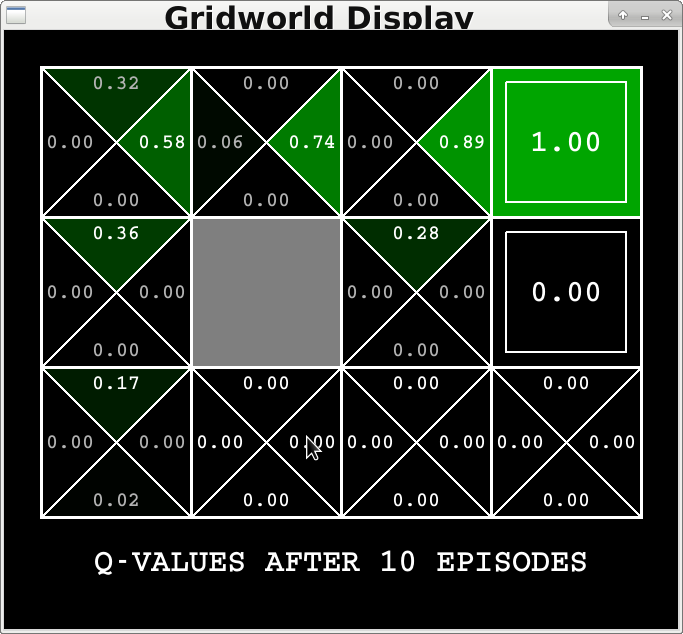
\includegraphics[width=\textwidth]{./images/qlearning_gridworld_10}
			\caption{\(Q\)-learning agent \(Q\) values}
		\end{subfigure}%
		\begin{subfigure}[b]{0.25\textwidth}
			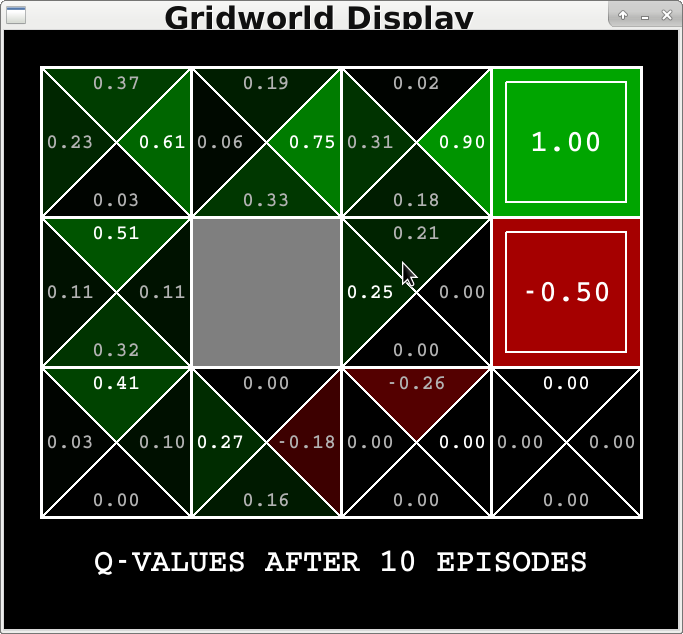
\includegraphics[width=\textwidth]{./images/sarsa_gridworld_10}
			\caption{Sarsa\((\lambda)\) agent \(Q\) values}
		\end{subfigure}
		\caption{\(Q\) values of the \(Q\)-learning and Sarsa\((\lambda)\) agents 
		after 10 episodes of training.  The Sarsa\((\lambda)\) agent is able
		to evaluate more of the state space than the \(Q\)-learning agent.
		Each agent was run for 10 episodes on the BookGrid world with a noise
		rate of 0.2, and \(\epsilon = 0.5\).}
		\label{qvalues}
	\end{figure}

	\begin{figure*}[h]
		\centering
		\begin{subfigure}[b]{0.40\textwidth}
			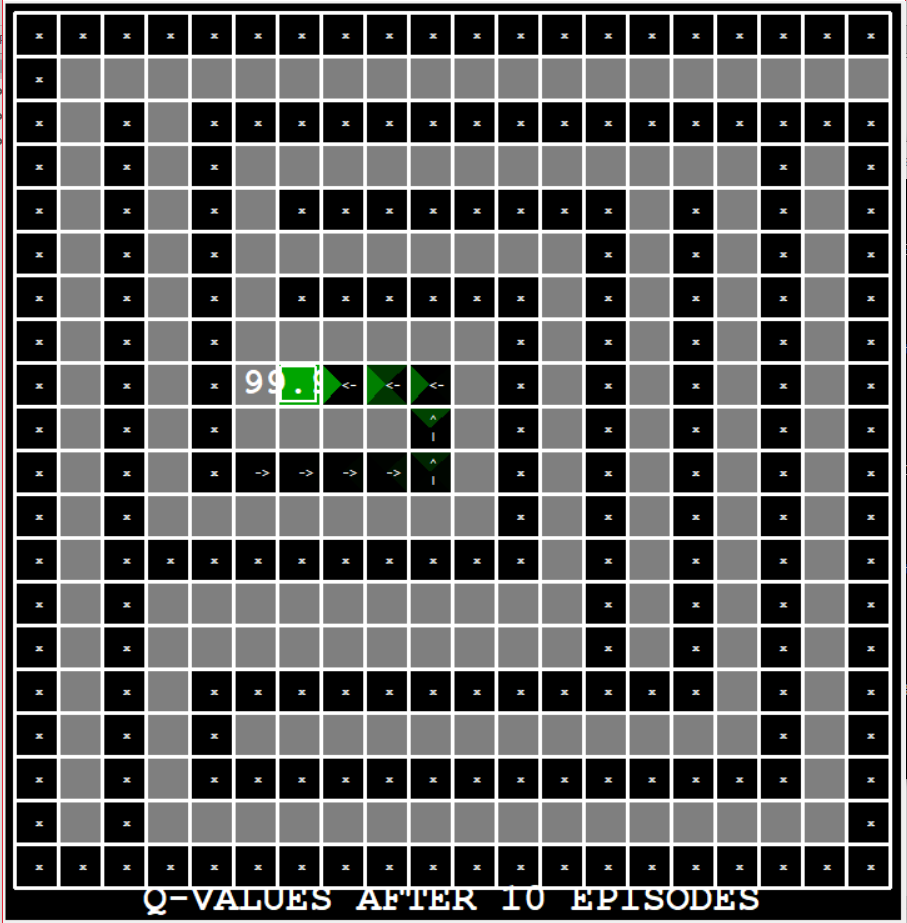
\includegraphics[width=\textwidth]{./images/qlearning_largeMaze_10}
			\caption{\(Q\)-learning agent Policy}
		\end{subfigure}%
		\begin{subfigure}[b]{0.40\textwidth}
			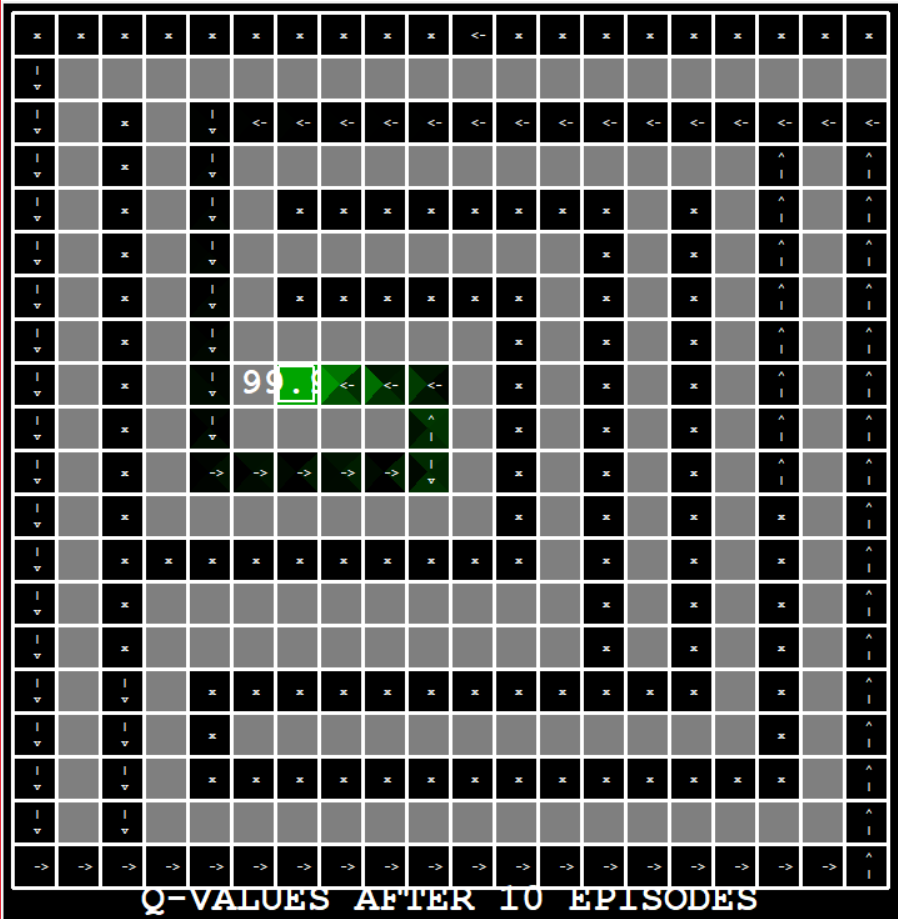
\includegraphics[width=\textwidth]{./images/sarsa_largeMaze_10}
			\caption{Sarsa\((\lambda)\) agent Policy}
		\end{subfigure}
		\caption{Policies of the \(Q\)-learning and Sarsa\((\lambda)\) agents 
		after 10 episodes on the LargeMazeGrid. Sarsa\((\lambda)\) agent's policy is almost on the verge of converging as opposed to that of the \(Q\)-learning agent.}
		\label{qvalues}
	\end{figure*}

		\begin{figure}[h]
		\centering
		\begin{subfigure}[b]{0.25\textwidth}
			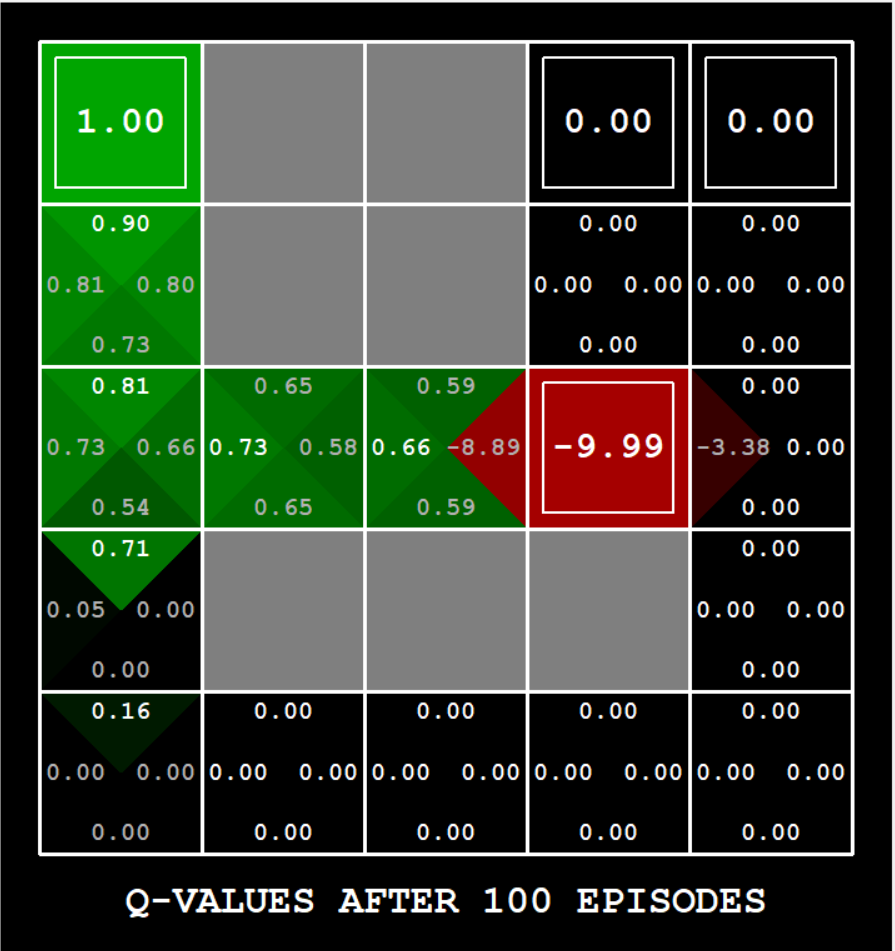
\includegraphics[width=\textwidth]{./images/qlearning_customGrid_100}
			\caption{\(Q\)-learning agent \(Q\) values}
		\end{subfigure}%
		\begin{subfigure}[b]{0.25\textwidth}
			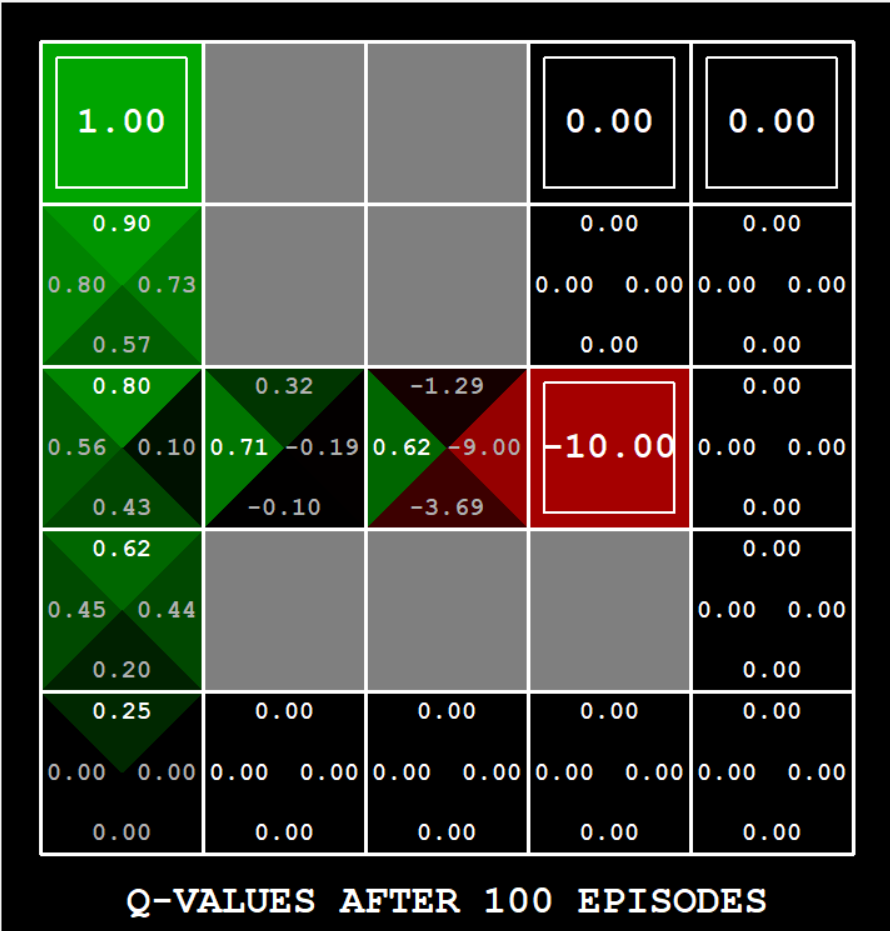
\includegraphics[width=\textwidth]{./images/sarsa_customGrid_100}
			\caption{Sarsa\((\lambda)\) agent \(Q\) values}
		\end{subfigure}
		\caption{\(Q\) values of the \(Q\)-learning and SARSA\((\lambda)\) agents 
		after 100 episodes on the CustomGrid. Identical results are found for both the agents on this grid.}
		\label{qvalues}
	\end{figure}

	In the \textit{gridworld.py} experiments we found that SARSA\((\lambda)\) 
	performed better per episode than \(Q\)-learning due its eligibility trace allowing for
	each training episode to update more of the \(Q\)-values than \(Q\)-learning's
	single step functions. Figure \ref{qvalues} clearly illustrates the difference. 
	After only 10 training episodes, a majority of the \(Q\)-values have been
	updated at least once by the SARSA\((\lambda)\) agent; while the \(Q\)-learning
	agent has only updated a few of its \(Q\)-values.

	The ability to update the \(Q\)-values associated with each \((state,action)\) 
	in the eligibility trace allows for good decisions be effect the value of the 
	prior decisions, and thus speeds up policy convergence.  It also, means that
	SARSA\((\lambda)\) is susceptible to noise, as a series of poor or random choices 
	that lead to a positive outcome are \textit{all} updated as though those 
	decisions were good or meaningful to the final outcome.  This leads the agent
	to get temporarily stuck in policies which are not optimal, meaning take longer
	to achieve the goal.

	\begin{figure*}[h]
		\centering
		\begin{subfigure}{0.40\textwidth}
			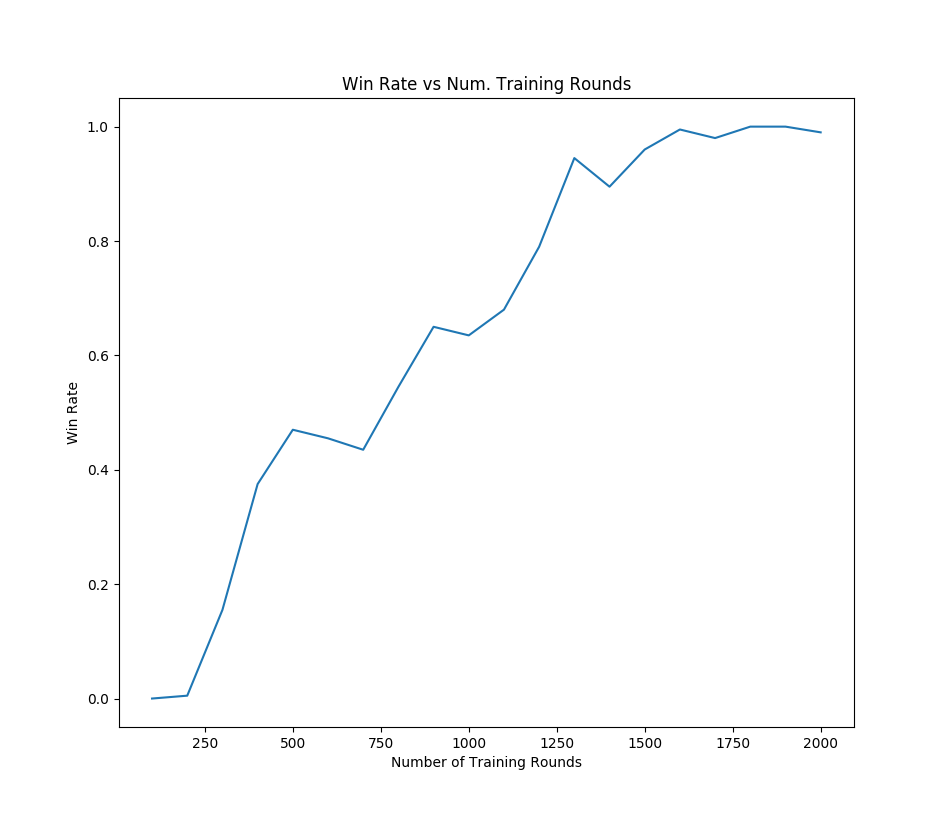
\includegraphics[width=\textwidth]{./images/qlearning_winrate}
			\caption{\(Q\)-Learning Agent}
		\end{subfigure}%
		\begin{subfigure}{0.40\textwidth}
			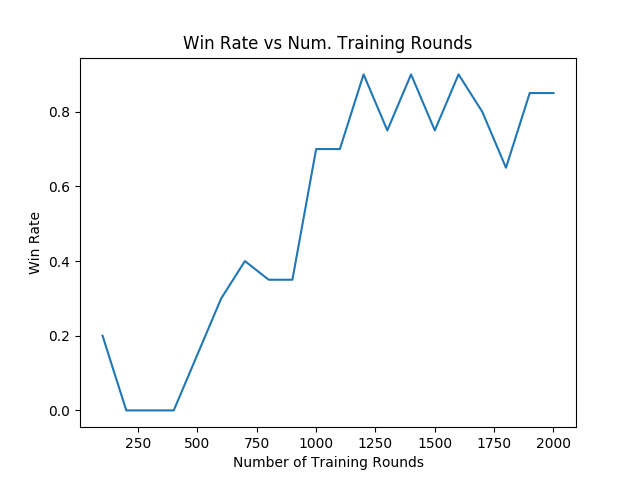
\includegraphics[width=\textwidth]{./images/sarsa_winrate}
			\caption{Sarsa\((\lambda)\) Agent}
		\end{subfigure}
		\caption{Win rate vs training episodes for \(Q\)-learning and
		Sarsa\((\lambda)\) agents.  Each agent was trained using 
		pacman smallGrid environment.  Win rate was taken from 
		20 post training episodes. Each agent was trained with 
		\(\epsilon = 0.05, \gamma = 0.8, \alpha = 0.2\).  The 
		Sarsa\((\lambda)\) agent has a default \(\lambda = 0.8\).}
		\label{winrate}
	\end{figure*}

	The other trade off of using the eligibility trace each time the agent 
	picks an action, is the time needed to loop through all of the \(Q\)-values
	visited in the environment. For small simple environments such as \textit{gridworld.py},
	the trade off between training time and number of training episodes puts 
	SARSA\((\lambda)\) ahead of \(Q\)-learning. However, in the more complex 
	\textit{pacman.py} environment the SARSA\(\lambda)\) agent slows down 
	considerably. Even though Figure \ref{winrate} shows that SARSA\((\lambda)\) 
	was able to reach peak win rate with fewer training episodes than \(Q\)-learning,
	the difference in real world training time was several hours.

\section{Conclusion}
From what we have already implemented, we can easily draw two conclusions:

1. \(Q\)-learning maybe suffers from problems converging as a result due to it has higher per-sample variance than SARSA\((\lambda)\), however SARSA\((\lambda)\) learns a near-optimal policy while exploring. So if we decide to use SARSA\((\lambda)\), we need propose a good strategy to explore alternative paths, as might occur with \(\epsilon\)-greedy action choice, which can become fiddly hyper parameter to adjust.

2. SARSA\((\lambda)\) is more conservative than \(Q\)-learning, because SARSA will approach convergence allowing for all kinds of penalties while agent explores its move while the \(Q\)-learning ignore them. In another words, if there is risk of a large negative reward close to the optimal path, Q-learning will react more aggressively and will avoid the area associated with that risk. On the contrary, SARSA\((\lambda)\) will try to avoid it and slowly learn to use it.

3. When both algorithms use linear function approximation, \(Q\)-learning converges faster than SARSA\((\lambda)\) but at the end of the training SARSA\((\lambda)\) seems to have a winrate of 1.0 as opposed to LFA \(Q\)-learning, which is high, but doesn't remain at 1.0.

\(Q\)-learning seems to learn at a far lower computational cost per episode, but SARSA\((\lambda)\) converges faster each episode, implying that if you are doing machine learning in the real world, 
where episodes can take a comparatively very long time, SARSA\((\lambda)\) should be your choice over \(Q\)-learning.

However, with LFA, SARSA\((\lambda)\)'s performance per episode drastically decreases. The plateau at 1.0 success rate at the end of the graph suggests that it may still be desireable if the above is true and a .01 failure rate is unacceptable, but \(Q\)-learning with LFA will perform far better in fewer episodes, and perhaps orders of magnitude less computational cost.

\label{sec:conclusion}

\section{Team Effectiveness}
We met soon after the team project was assigned, all having done the related homework, and done the SARSA\((\lambda)\) algorithm. Building the team had been a somewhat slow process, but we managed to find each other and put us all in one group chat, which was a wise decision as now we were all able to communicate instantly and directly with one another. In the meeting, we decided what our general roles would be, and set to work. Despite our team chat, however, we still had minor communication issues, as some of us missed the messages one way or another. Our biggest mistake was not misunderstanding the instructions, setting out to describe the differences of SARSA\((\lambda)\) and \(Q\)-learning without LFA. Luckily, we were able to spot our mistake, and run some tests displaying how the 2 compare with FLA.
\label{sec:team}


\bibliographystyle{abbrv}
\bibliography{ref}
\end{document}












